%-----------------------------------LICENSE------------------------------------%
%   This file is part of tikz_figures.                                         %
%                                                                              %
%   tikz_figures is free software: you can redistribute it and/or              %
%   modify it it under the terms of the GNU General Public License as          %
%   published by the Free Software Foundation, either version 3 of the         %
%   License, or (at your option) any later version.                            %
%                                                                              %
%   tikz_figures is distributed in the hope that it will be useful,            %
%   but WITHOUT ANY WARRANTY; without even the implied warranty of             %
%   MERCHANTABILITY or FITNESS FOR A PARTICULAR PURPOSE.  See the              %
%   GNU General Public License for more details.                               %
%                                                                              %
%   You should have received a copy of the GNU General Public License along    %
%   with tikz_figures.  If not, see <https://www.gnu.org/licenses/>.           %
%------------------------------------------------------------------------------%

% Use the standalone class for displaying the tikz image on a small PDF.
\documentclass[crop, tikz]{standalone}

% Import the tikz package to use for the drawing.
\usepackage{tikz}

% Begin the document.
\begin{document}

    % Draw the figure.
    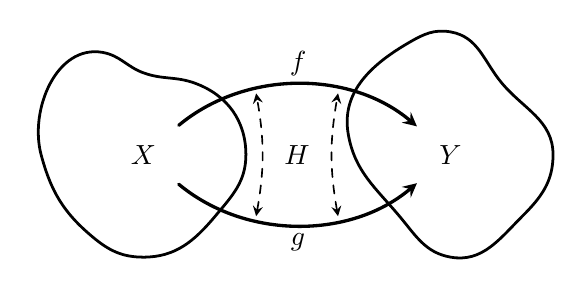
\begin{tikzpicture}[%
        scale = 1.3,
        line width = 1pt,
        line cap = round,
        > = stealth,
        every edge/.style = {%
            draw = black,
            very thick
        },
        smalldot/.style = {
            circle,
            fill = black,
            inner sep = 0pt,
            outer sep = 0
        }
    ]

        % Set points defining the leftmost blob.
        \coordinate (a) at (0.0, 0.0);
        \coordinate (b) at (-0.5, 0.2);
        \coordinate (c) at (-1.0, 1.0);
        \coordinate (d) at (-0.4, 2.0);
        \coordinate (e) at (0.0, 1.8);
        \coordinate (f) at (0.5, 1.7);
        \coordinate (g) at (1.0, 1.0);
        \coordinate (h) at (0.7, 0.4);

        % Set points defining the rightmost blob.
        \coordinate (a1) at (3.0, 0.0);
        \coordinate (b1) at (2.5, 0.4);
        \coordinate (c1) at (2.0, 1.2);
        \coordinate (d1) at (2.6, 2.1);
        \coordinate (e1) at (3.0, 2.2);
        \coordinate (f1) at (3.5, 1.7);
        \coordinate (g1) at (4.0, 1.0);
        \coordinate (h1) at (3.7, 0.4);

        % Labels for the blobs X and Y.
        \node at (0.0, 1.0) (i) {$X$};
        \node at (3.0, 1.0) (i1) {$Y$};

        % Node indicating this is a homotopy.
        \node at (1.5, 1.0) (ho) {$H$};

        % Nodes for drawing arrows between curves.
        \coordinate (t1) at (1.1, 0.4);
        \coordinate (t2) at (1.1, 1.6);
        \coordinate (t3) at (1.9, 0.4);
        \coordinate (t4) at (1.9, 1.6);

        % Draw a Hobby curve creating leftmost blob.
        \draw (a) to [out = 180, in = -40]
              (b) to [out = 140, in = -75]
              (c) to [out = 105, in = 170]
              (d) to [out = -10, in = 160]
              (e) to [out = -20, in = 160]
              (f) to [out = -20, in = 90]
              (g) to [out = -90, in = 50]
              (h) to [out = -130, in = 0] cycle;

        % Draw Hobby curve creating rightmost blob.
        \draw (a1) to [out = 170, in = -50]
              (b1) to [out = 130, in = -80]
              (c1) to [out = 100, in = -150]
              (d1) to [out = 30, in = 170]
              (e1) to [out = -10, in = 130]
              (f1) to [out = -50, in = 90]
              (g1) to [out = -90, in = 45]
              (h1) to [out = -135, in = -10] cycle;

        % Draw arrows representing f and g.
        \begin{scope}[%
            shorten > = 0.2cm,
            shorten < = 0.2cm,
            ->
        ]
            \path (i) edge[bend left = 40] node[above] {$f$} (i1);
            \path (i) edge[bend right = 40] node[below] {$g$} (i1);
        \end{scope}

        \begin{scope}[%
            draw = black,
            dashed,
            <->
        ]
            % Draw first arrow connecting f and g.
            \path (t1) edge[bend right = 10, semithick] (t2);

            % Draw second arrow connecting f and g.
            \path (t3) edge[bend left = 10, semithick] (t4);
        \end{scope}
    \end{tikzpicture}
\end{document}
